%!TEX root = ../main.tex

\section{Preliminaries}
\label{sec:prelim}

We assume countable sets $\mathcal{R}$ of unary and binary relation 
 names and an $\mathcal{C}$ of constants. 
A \emph{knowledge graph} (KG) $\G$ is a finite set of ground atoms $a$ of the form
$R(a,b)$ and $C(a)$ over the $\R\cup\C$.
With $\Sigma_{\cG}$ we denote those elements of $\R\cup\C$ that occur in $\G$
and refer to it as the \emph{signature} of $\G$.


We define rules over KGs following the standard approach of non-monotonic logic programs under the answer set semantics, see e.g. \cite{GL1988}.
Let $\X$ be a countable set of variables.
A \emph{rule} $r$ is an expression of the form
$
\mi{head \leftarrow body},
$
where $\mi{head}$, or $\mi{head}(r)$, is an antom 
%of the form $a(\vec{X})$ 
over $\R\cup\C\cup\X$ 
%and $\vec{X}$ are its variables,
and $body$, or $\mi{body}(r)$, is a conjunction of positive and negative atoms 
over $\R\cup\C\cup\X$.
We also denote with $\mi{body^+(r)}$ and $\mi{body^-(r)}$ the positive and 
negative atoms of $r$.

We define \emph{execution} of rules over KGs in the standard way using default negation~\cite{GL1988}.
More precisely, let $\G$ be a KG, $r$  rule over $\Sigma_\G$, 
and $a$ be an atom over $\Sigma_G$.
Then, $r \models_\G a$ holds if there is a variable assignment $h$ that maps  atoms $\mi{body^+(r)}$ in $\G$ such that it does not map any of the atoms in $\mi{body^-(r)}$ in $\G$. 
%\evgeny{Is this correct?}
Then, let $\G_r = \G \cup \set{a \mid r \models_\G a}$. 

\evgeny{this should be enough for the preliminaries}

\leanparagraph{Knowledge graphs} On the Web, knowledge graphs (KG) are often encoded using the RDF data
model~\cite{rdf}, which represents the content of the graph with a set of
triples of the form $\tuple{\mi{subject}\;\mi{predicate}\;\mi{object}}$, reflecting positive unary (e.g., $\mi{\tuple{bob\;type\;scientist}}$) and binary (e.g., $\tuple{\mi{bob\;livesIn\;rome}}$) facts about the world naturally treated under the Open World Assumption (OWA).  %which also known as facts.
% These triples encode
%positive facts about the world, and they are naturally treated under the open world assumption (OWA).


%In this work, we focus on KGs without blank nodes or schema (TBox in the OWL
%terminology). 
%For simplicity, we represent the triples using binary
%predicates. 
We %call this the
%factual representation of the 
consider KGs $\cG$ defined over the signature
$\Sigma_{\cG}=\tuple{\mathcal{R},\mathcal{C}}$, where $\mathcal{R}$ and $\mathcal{C}$ are sets of
relations and constants respectively. 
%E.g., %$\tuple{\mi{alice\;isA\;researcher}}$ in $\cG$ corresponds to $\mi{researcher(alice)}$,  
%$\tuple{\mi{bob \;isMarriedTo\;alice}}$ corresponds to $\mi{isMarriedTo(bob,alice)}$ in the factual representation. 

% Relying on \cite{DBLP:conf/semweb/DarariNPR13} we define the gap between the ideal graph %The ideal graph 
% $\cG^i$ (a graph containing all possible correct facts with constant and relation from $\Sigma_{\cG}$) and the available graph $\cG^a$. 
% %Thus, we define the incomplete actual graph $\cG^a$ as 

% \begin{definition}[Incomplete data source] An incomplete data source is a pair
%     $G = (\cG^a, \cG^i)$ of two KGs, where $\cG^a\subseteq \cG^i$ and
%     $\Sigma_{\cG^a}=\Sigma_{\cG^i}$. 
% \end{definition}


\leanparagraph{Rules}
We consider logic programs under the answer set semantics defined as usual \cite{GL1988}.
%logic program in the standard way~\cite{DBLP:books/sp/Lloyd87}. 
In short, a \emph{(nonmonotonic) logic program} $P$ is a set of \emph{rules} $r$ of the form
\begin{equation}
H\leftarrow B, \naf E
\end{equation}
\noindent where $H$ is a standard first-order atom of the form $a(\vec{X})$ known as the rule head and denoted as $\mi{head(r)}$, $B$ is a conjunction of positive atoms of the form $b_1(\vec{Y_1}),\dotsc,b_k(\vec{Y_k})$ to which we refer as $\mi{body^+(r)}$ and $\naf\ E$, with slight abuse of notation, denotes the conjunction of atoms $\naf\, b_{k+1}(\vec{Y_{k+1}}),\dotsc,\naf\, b_n(\vec{Y_{n}})$, where $\naf$ is called \emph{negation as failure (NAF)} or \emph{default negation}.
Here, $\vec{X},\vec{Y_1},\ldots,\vec{Y_{n}}$ are tuples of either constants or
variables whose length corresponds to the arity of the predicates
$a,b_1,\ldots,b_n$ respectively. The signature of $P$ is given as $\Sigma_{\mi{P}}=\tuple{\mathbf{P},\cC}$, where $\mathbf{P}$ and $\cC$ are sets of predicates and constants occurring in $P$ respectively. %Positive, negative body and head of a rule $r$ are defined as usual \cite{DBLP:books/sp/Lloyd87} and denoted resp. as $B^+(r),B^-(r)$ and $H(r)$.

%We consider answer set semantics in this work, see \cite{GL1988} for details.

\leanparagraph{Classical rule measures}
Association rule learning concerns the discovery of frequent patterns in a data set and the subsequent transformation of these patterns into rules.
A \emph{conjunctive query} $Q$ over $\cG$ is of the form $Q(\vec{X}) \text{ :- } p_1(\vec{X_1}),\dotsc,p_m(\vec{X_m})$, where $\vec{X_i}$ are binary vectors of variables. Its  right-hand side (i.e., body) is a finite set of atomic formulas over $\Sigma_{\cG}$, while the left-hand side (i.e., head) is a tuple of variables occurring in the body. The \emph{answer} of $Q$ on $\cG$ is the set $Q(\cG) = \{ \nu(\vec{X}) \mid \nu \text{ is a function from variables to } \mathcal{C} \text{ and } \forall i: p_i(\nu(\vec{X_i})) \in \cG \}$.
%As in \cite{DBLP:conf/ilp/DehaspeR97}, t
The \emph{support} of
$Q$ in $\cG$ is the number of distinct tuples in the answer of $Q$ on $\cG$. 

An \emph{association rule} is of the form $Q_1 \Rightarrow  Q_2$, such that $Q_1$ and $Q_2$ are both conjunctive queries and $Q_1 \subseteq Q_2$, i.e., $Q_1(\cG')\subseteq Q_2(\cG')$ for any possible KG $\cG'$. In this work we exploit association rules for reasoning purposes, and thus (with some abuse of notation) treat them as logical rules, i.e., for $Q_1\Rightarrow Q_2$ we write $Q_2\backslash Q_1 \leftarrow Q_1$, where $Q_2 \backslash Q_1$ refers to the set difference between $Q_2$ and $Q_1$ seen as sets of atoms.
\begin{figure}[tb]
\centering
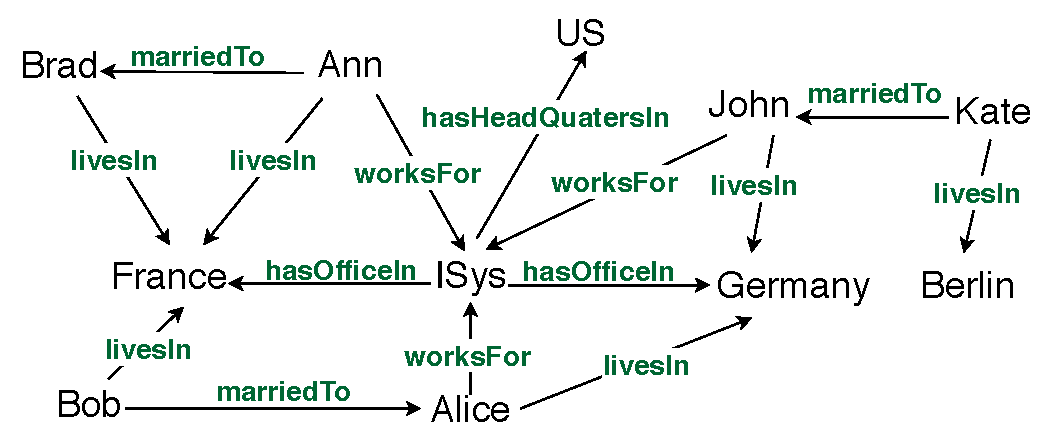
\includegraphics[width=.5\textwidth]{figures/kg3.pdf}
%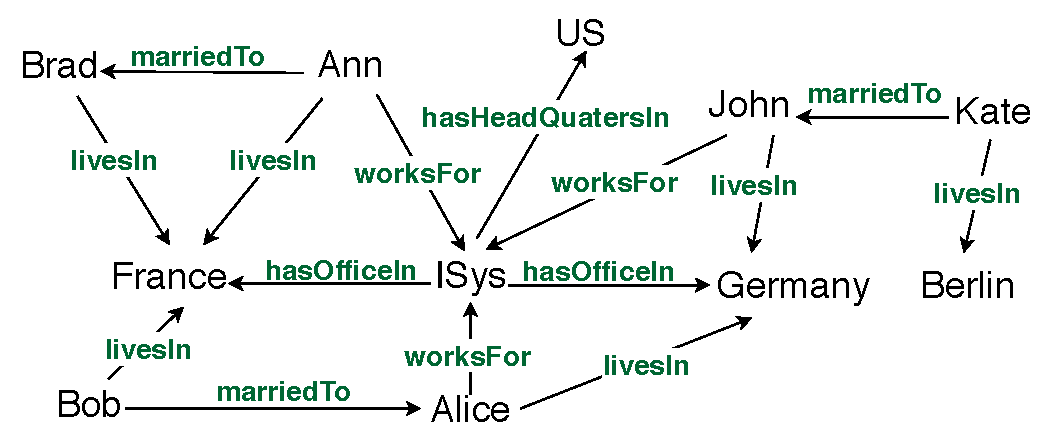
\includegraphics[scale=0.32]{figures/kg3.pdf}
\caption{An example KG where red-dashed arrows are missing relations.}
\label{fig:kg}
\end{figure}
Classical scoring of association rules is based on \emph{rule support}, \emph{body support}, \emph{confidence} and \emph{PCA confidence}, which in \cite{amie} for
% a rule
$r:\mi{h(x,y)\,{\leftarrow}\,\vec{B}}$
are defined as:
%
\begin{equation}\label{eq:supp}
\mi{supp}(r) := \#(x,y): \exists \vec{Z}: \vec{B} \wedge h(x,y)
\end{equation}
\begin{equation}\label{eq:body_supp}
\mi{supp}(\vec{B}) := \#(x,y): \exists \vec{Z}: \vec{B}
\end{equation}
\begin{equation}\label{eq:std_conf}
\mi{conf}(r) := \frac{\mi{supp}(r)}{\mi{supp}(\vec{B})}
\end{equation}
\begin{equation}\label{eq:pca_conf}
\mi{conf_{pca}}(r) := \frac{\mi{supp}(r)}{\#(x,y): \exists \vec{Z}: \vec{B} \wedge \exists y': h(x,y')\in \cG^a}
\end{equation}
where $\# \alpha : \mathcal{A}$ denotes the number of $\alpha$ that fulfill the condition $\mathcal{A}$.

\begin{example}
Consider the KG in Fig. \ref{fig:kg} and the rules $r_1$ and $r_2$ from Section~\ref{sec:intro}% :\\
% \textit{ - $r_1$ : livesIn(X,Z) $\leftarrow$ marriedTo(X,Y), livesIn(Y,Z)}\\
% \textit{ - $r_2$ : livesIn(X,Z) $\leftarrow$ worksAt(X,Y), hasOfficeIn(Y,Z)}\\
% With $r_1$, the rule and body supports over the KG are
. For $r_1$ we have $supp(\vec{B})=8$ and
$supp(r_1) = 5$, thus % , correspondingly.
% Hence, we have
$conf(r_1) = conf_{pca}(r_1)=\frac{5}{8}$ % and  % Additionally % we also have
% $conf_{pca}(r_1) = \frac{5}{8}$, since we do not know where \textit{Kate} lives. 
For $r_2$, we have $\mi{conf(r_2) =} \frac{2}{6}$ and $\mi{conf_{pca}(r_2) =}\frac{2}{4}$, since Julia's and Robin's living places are unknown. Similarly, we have $\mi{conf(r_3) =} \frac{2}{5}$ and $\mi{conf_{pca}(r_3) =}\frac{2}{4}$.
\qed
\end{example}

Given a rule $r$ and a KG $\cG$ the application of $r$ on $\cG$ results in a rule-based graph completion defined relying on the Answer Set semantics.

% \begin{definition}[Rule-based KG completion]\label{def:graphcompl}
% Let $\cG$ be a KG over the signature $\Sigma_{\cG}=\tuple{\mathbf{R},\cC}$ and let $r$ be a rule %$r$ be a set of rules 
% mined from $\cG$, i.e. a rule over $\Sigma_{\cG}$.
% Then the \emph{completion of $\cG$} using rule $r$ is a graph $\cG_{r}$ constructed from any answer set of $r \cup \cG$. 
% \end{definition}

% % \begin{example}
% % The application of $r_1$ and $r_2$ on $\cG^a$ from Fig. \ref{fig:kg} results in:\\
% % \textit{ - $\cG^a_{r_1} = \cG^a\;\cup$ \{livesIn(James,Paris), livesIn(Kann,France), livesIn(Lisi,Italy)\}}\\
% % \textit{ - $\cG^a_{r_2} = \cG^a\;\cup$ \{livesIn(James,Paris), livesIn(Kann,Rome), livesIn(Alice,Paris), livesIn(Lisi,Paris)\}}. \qed
% % \end{example}

%  \begin{example}
%  The application of $r_1$, $r_2$ and $r_3$ on $\cG^a$ from Figure~\ref{fig:kg} results in:
% \begin{itemize}
% \item ${\cG^a_{r_1}}{=}\cG^a\cup\{\mi{livesIn(ann{,}chicago),livesIn(john{,}berlin),livesIn(kate{,}china)}\}$
% \item ${\cG^a_{r_2}}{=}\cG^a\cup\{\mi{livesIn(julia{,}chicago),livesIn(clara{,}us),livesIn(robin{,}berlin),}\\
% \mi{livesIn(kate{,}chicago)}\}$
% \item ${\cG^a_{r_3}}{=}\cG^a\cup\{\mi{livesIn(clara{,}us),livesIn(robin{,}berlin),livesIn(kate{,}chicago)}\}$
% \end{itemize}
% \qed
%  \end{example}

Note that $\cG^i$ is the perfect completion of $\cG^a$, i.e., it is supposed to contain all
correct facts with entities and relations from $\Sigma_{\cG^a}$ that hold
in the current state of the world. The goal of rule-based KG completion is to extract from $\cG^a$ a set of rules $\cR$ such that $\cup_{r\in \cR}\cG^a_{r}$ is as close to $ \cG^i$ as possible.

\leanparagraph{Link prediction embedding models} Recently a vast amount of translation-based approaches for statistical relational learning have been proposed  (see \cite{DBLP:journals/tkde/WangMWG17} for overview), which address the KG completion problem by reducing it to a representation learning task, where the main goal is to represent entities and relations of $\cG$ in a
low-dimensional, say $d$-dimensional, vector (aka embedding) and relying on these representation estimate the likelihood of the potentially missing facts. 
%vector space $\vec{h}, \vec{t}, \vec{r} \in I\!R^d$ such that for $\tuple{h,r,r}\in \cG$ it holds that $\vec{h}+\vec{r}\approx \vec{t}$.  
Some models  exclusively make use of the triples in the available KG and estimate the likelihood of the missing ones~\cite{Bordes:2013:TEM:2999792.2999923,DBLP:conf/aaai/NickelRP16}, while others may utilize external sources (\eg text)~\cite{DBLP:conf/aaai/0005HMZ17}. 

%For a pair $\tuple{\cG, \cE}$, $\cE$ is an embedding model of $\cG$, if for each triple $\tuple{s,p,o}\in \cG$, there exists a vector $v \in \cE$. 
Typical embedding models define a scoring function $score_e: \cR \times \cC \times \cC  \rightarrow {\rm I\!R}$ 
%\thi{not necessary between 0-1, the inverted rank is using is between 0-1, not the original embedding scoring function}
that given an $\tuple{\mi{s\;p\;o}}$ triple computes a numerical value reflecting its likelihood. % The higher is the plausibility score, the more likely the fact $\tuple{s,p,o}$ is true.
E.g., TransE \cite{Bordes:NIPS2013} model defines the scoring function as follows:
\[score_e(p(s,o)) = -||E_s + R_p - E_o||_{l_{1,2}}\]
where $E_s$, $R_p$, $E_o$ are the embeddings of subject, predicate and object, respectively.

% Apart from asking for the plausibility score of an individual fact $\tuple{s,p,o}$, the existing embedding models can also output a list of ordered potential objects given $\tuple{s,p,?}$ by ranking them based on the plausibility score. Other two other types of potential queries include $\tuple{?,p,o}$ and $\tuple{s,?,o}$, and they are treated similarly.

%The plausibility score of $f_e(\tuple{s,p,o})$ %of 
%to a plausible triple 
%should be higher for $\tuple{s,p,o}\in \cG$ then for  %than %the score $f_e(\tuple{s',p',o'})$ of  the 
% $\tuple{s,p,o}\not \in \cG$~\cite{kazemi2017comparing}.

While in this work we experiment with several selected KG embedding models, our general rule learning approach can conceptually exploit any model or even there combination as we explain in Section~\ref{sec:method}. %If we treat a KG embedding model as an oracle, then the questions that one can pose to it include $\tuple{s,p,o}$, $\tuple{s,p,?}$, $\tuple{?,p,o}$ and $\tuple{s,?,o}$.
% \begin{example}

% \end{example}
%with a list of pairs $(\tuple{s',p',o'},s)$ where $\tuple{s',p',o'}$ is matchable with the query triple and score $s\in {\rm I\!R}$  representing implausibility of the resulting triple.



